\chapter[Настройка]{Настройка \cg{}}
\label{chap:setting_up_your_cg6_autograv}

Гравиметр \cg{} имеет дополнительный планшетный компьютер (номер по каталогу
888030), который позволяет пользователю быстро настроить и спланировать съёмку с
помощью предварительно загруженного программного обеспечения LynxLG.
Пожалуйста, обратитесь к Руководству по программному обеспечению LynxLG
Acquisition (p/n 115370003) для получения дополнительной информации о настройке
с помощью планшетного компьютера.

\infobox{
  Вы можете управлять работой прибора \cg{} как с помощью планшетного компьютера
  (\textnumero{} 888030), так и без него. Прибор \cg{} снабжён программным
  обеспечением и пользовательским интерфейсом, который позволяет пользоваться
  прибором как полнофункциональным автономным гравиметром. Режим планшетного
  компьютера предоставляет вам больше возможностей и позволяет дистанционно
  управлять работой прибора \cg{}. Кроме того, в этом режиме пользователю
  предоставляется доступ к расширенным функциональным возможностям, таким,
  например, как создание координатных карт пунктов наблюдения для определения
  местоположения в реальном времени, средства импорта пунктов
  наблюдения/маршрута (KML, GPX, Delimited ASCII), и создание простых карт
  редукций Буге.
}

\section{Меню настроек Settings}

На главном экранном изображении наведите курсор на пункт \textbf{SETTINGS}
(изображение внизу слева) и нажмите кнопку \textbf{Enter}. Откроется экран,
показанный справа:

\newpage
\begin{figure}[H]
  \centering
  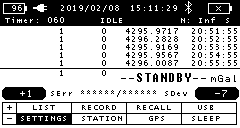
\includegraphics[width=0.49\textwidth]{figures/the_settings_screen_1}
  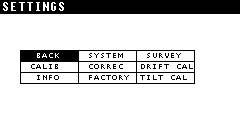
\includegraphics[width=0.49\textwidth]{figures/the_settings_screen_2}
  \caption{Экран меню настроек}
  \label{fig:the_settings_screen}
\end{figure}

\section{Настройка системы}

Чтобы получить доступ к экранному изображению настроек системы, наведите курсор
на пункт \textbf{SYSTEM} (изображение внизу слева) и нажмите кнопку
\textbf{Enter}.  Откроется экран, показанный справа:

\begin{figure}[H]
  \centering
  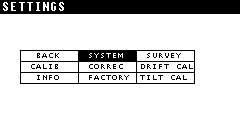
\includegraphics[width=0.49\textwidth]{figures/the_system_screen_1}
  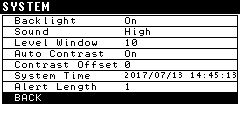
\includegraphics[width=0.49\textwidth]{figures/the_system_screen_2}
  \caption{Экран системы}
  \label{fig:the_system_screen}
\end{figure}

\subsection{Включение и выключение фоновой подсветки экрана}

Фоновая подсветка экрана может находиться в одном из двух состояний: ON или OFF.
Для настройки фоновой подсветки наведите курсор на пункт \textbf{Backlight}
(изображение внизу слева) и нажмите кнопку \textbf{Enter}. Откроется экран,
показанный справа:

\newpage
\begin{figure}[H]
  \centering
  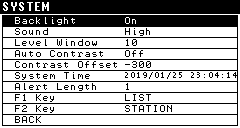
\includegraphics[width=0.49\textwidth]{figures/the_backlight_screen_1}
  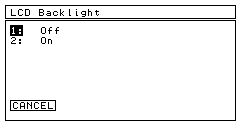
\includegraphics[width=0.49\textwidth]{figures/the_backlight_screen_2}
  \caption{Экран настройки фоновой подсветки}
  \label{fig:the_backlight_screen}
\end{figure}

Фоновую подсветку можно включить (\textbf{On}) или выключить (\textbf{Off}).
Наведите курсор на символ 1 или 2 и нажмите кнопку \textbf{Enter}.

Чтобы покинуть это экранное изображение без изменений:
\begin{itemize}
  \item наведите курсор на пункт \textbf{CANCEL}, после чего нажмите кнопку
    \textbf{Enter}, или

  \item нажмите кнопку \textbf{Back}
\end{itemize}

\subsection{Настройка громкости звукового сигнала}

Для громкости звукового сигнала предусмотрено четыре варианта выбора: Low
(Низкая), Medium (Средняя), High (Высокая) или Disabled (Отключена). Для
настройки громкости наведите курсор на пункт \textbf{Sound} (изображение внизу
слева) и нажмите кнопку \textbf{Enter}. Откроется экран, показанный справа:

\begin{figure}[H]
  \centering
  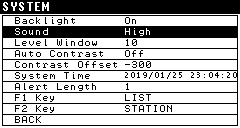
\includegraphics[width=0.49\textwidth]{figures/the_buzzer_volume_screen_1}
  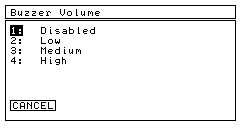
\includegraphics[width=0.49\textwidth]{figures/the_buzzer_volume_screen_2}
  \caption{Экран настройки громкости звукового сигнала}
  \label{fig:the_buzzer_volume_screen}
\end{figure}

Наведите курсор на пункт, соответствующий нужной громкости, и нажмите кнопку
\textbf{Enter}.

Чтобы покинуть это экранное изображение без изменений:
\begin{itemize}
  \item наведите курсор на пункт \textbf{CANCEL}, после чего нажмите кнопку
    \textbf{Enter}, или

  \item нажмите кнопку \textbf{Back}
\end{itemize}

\subsection{Регулировка окна горизонтирования}
\label{subsec:adjusting_the_level_window}

\infobox{
  Величина окна горизонтирования~-- это порог, ниже которого цвет стрелок
  горизонтирования становится зелёным.  Например, если интервал горизонтирования задан
  равным 10 угловых секунд, тогда в случае, когда величина угла наклона одной из
  осей не выходит за пределы \textpm{}10 угловых секунд, соответствующая этой
  оси стрелка горизонтирования имеет зелёный цвет.
}

Для корректировки величины окна горизонтирования наведите курсор на пункт
\textbf{Level} \textbf{Window} (изображение внизу слева) и нажмите кнопку
\textbf{Enter}. Откроется экран, показанный справа:

\begin{figure}[H]
  \centering
  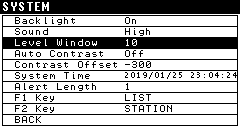
\includegraphics[width=0.49\textwidth]{figures/the_level_window_size_editing_screen_1}
  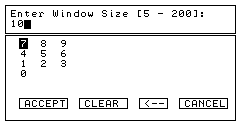
\includegraphics[width=0.49\textwidth]{figures/the_level_window_size_editing_screen_2}
  \caption{Экран выбора величины окна горизонтирования}
  \label{fig:the_level_window_size_editing_screen}
\end{figure}

Введите желаемый размер окна с помощью экранной клавиатуры, как описано в
разделе \nameref{subsubsec:entering_a_value_with_onscreen_keypad}.

\subsection{Включение/выключение автоматического изменения контрастности}

Функция автоматического изменения контрастности экранного изображения может
находиться в одном из двух состояний~-- ON или OFF. В общем случае, функция
автоматического изменения контрастности всегда должна быть включена. Тогда
регулирование контрастности будет осуществляться автоматически с учётом
температуры ЖК-дисплея. Это удобно при работе в поле, когда количество
солнечного света и внешняя температура могут сильно меняться в течение дня.
Чтобы включить или выключить функцию автоматического изменения контрастности
наведите курсор на пункт \textbf{Auto Contrast} (изображение внизу слева) и
нажмите кнопку \textbf{Enter}. Откроется экран, показанный справа:

\begin{figure}[H]
  \centering
  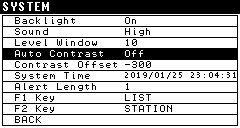
\includegraphics[width=0.49\textwidth]{figures/the_auto_contrast_screen_1}
  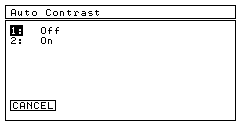
\includegraphics[width=0.49\textwidth]{figures/the_auto_contrast_screen_2}
  \caption{Экран функции автоматического изменения контрастности}
  \label{fig:the_auto_contrast_screen}
\end{figure}

Чтобы включить (\textbf{On}) или выключить (\textbf{Off}) функцию
автоматического изменения контрастности, наведите курсор на символ 1 или 2 и
нажмите кнопку \textbf{Enter}.

Чтобы покинуть это экранное изображение без изменений:
\begin{itemize}
  \item наведите курсор на пункт \textbf{CANCEL}, после чего нажмите кнопку
    \textbf{Enter}, или

  \item нажмите кнопку \textbf{Back}
\end{itemize}

\infobox{
  В общем случае, функция автоматического изменения контрастности всегда должна
  быть включена. Тогда регулирование контрастности будет осуществляться
  автоматически с учётом температуры ЖК-дисплея.
}

\subsection{Регулировка смещения контрастности экрана}

Помимо автоматической регулировки контрастности экранного изображения (см.
предыдущий раздел) вы также можете корректировать смещение контрастности (т.~е.,
яркость). Чем выше будет значение, тем темнее будет экранное изображение.  Для
редактирования величины смещения контрастности, наведите курсор на пункт
\textbf{Contrast Offset} (изображение внизу слева) и нажмите кнопку
\textbf{Enter}. Откроется экран, показанный справа:

\begin{figure}[H]
  \centering
  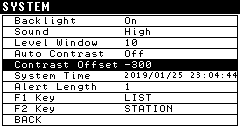
\includegraphics[width=0.49\textwidth]{figures/the_contrast_offset_editing_screen_1}
  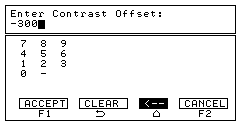
\includegraphics[width=0.49\textwidth]{figures/the_contrast_offset_editing_screen_2}
  \caption{Экран редактирования смещения контрастности}
  \label{fig:the_contrast_offset_editing_screen}
\end{figure}

Смещение контрастности может быть установлено на любое значение от -500 до
+1000.

Введите желаемое смещение контрастности с экранной клавиатуры, как описано в
разделе \nameref{subsubsec:entering_a_value_with_onscreen_keypad}

\infobox{
  Чем больше вводимая величина смещения контрастности, тем темнее будет ваше
  экранное изображение.
}

\subsection{Корректировка системных даты и времени}

\infobox{
  Вы можете ввести системные дату и время вручную, или синхронизировать их по
  GPS.
}

\subsubsection{Как ввести системные дату и время вручную}

Для корректировки системного времени, наведите курсор на пункт \textbf{System
  Time} (изображение внизу слева) и нажмите кнопку \textbf{Enter}. Откроется
экран, показанный справа:

\newpage
\begin{figure}[H]
  \centering
  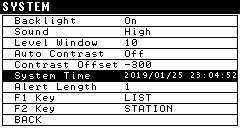
\includegraphics[width=0.49\textwidth]{figures/the_system_time_editing_screen_1}
  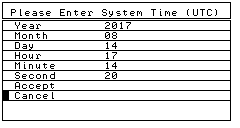
\includegraphics[width=0.49\textwidth]{figures/the_system_time_editing_screen_2}
  \caption{Экран редактирования системного времени}
  \label{fig:the_system_time_editing_screen_1}
\end{figure}

Чтобы ввести год, наведите курсор на пункт \textbf{Year} (год, изображение внизу
слева) и нажмите кнопку \textbf{Enter}. Откроется экран, показанный справа:

\begin{figure}[H]
  \centering
  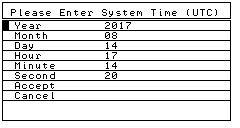
\includegraphics[width=0.49\textwidth]{figures/the_system_time_editing_screen_3}
  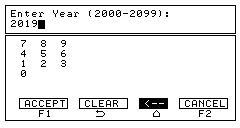
\includegraphics[width=0.49\textwidth]{figures/the_system_time_editing_screen_4}
  \caption{Экран редактирования системного времени}
  \label{fig:the_system_time_editing_screen_2}
\end{figure}

Введите значение года с помощью клавиатуры на экранной клавиатуре, как
описано в разделе \nameref{subsubsec:entering_a_value_with_onscreen_keypad}.

Повторите ту же процедуру для настройки месяца (month), дня (day), часа (hour),
минуты (minute) и секунды (second).

Чтобы принять новое значение системного времени, переместите курсор на
\textbf{Accept}
(на экране слева на рисунке~\ref{fig:the_system_time_editing_screen_2}) и
нажмите кнопку \textbf{Enter}.

\subsubsection{Обновление системных даты и времени при помощи встроенного блока
  GPS}

На главном экранном изображении наведите курсор на пункт \textbf{GPS} (изображение
внизу слева) и нажмите кнопку \textbf{Enter}. Откроется экран, показанный справа:

\begin{figure}[H]
  \centering
  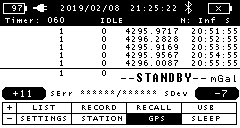
\includegraphics[width=0.49\textwidth]{figures/the_gps_screen_1}
  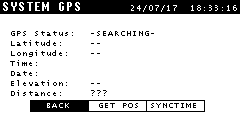
\includegraphics[width=0.49\textwidth]{figures/the_gps_screen_2}
  \caption{Экран GPS}
  \label{fig:the_gps_screen_1}
\end{figure}

\infobox{
  Поначалу статус блока GPS будет определён как <<SEARCHING>> (в процессе
  поиска).  Чтобы улучшить качество приёма сигнала, поместите прибор \cg{} в такое
  место, где он будет находиться под открытым небом.
}

После установления соединения статус блока GPS поменяется на <<LOCKED>> (Сигнал
захвачен). Поля Latitude (Широта), Longitude (Долгота), Time (Время), Date
(Дата), Elevation (Высота) и Distance (Расстояние) будут заполнены
автоматически.

Наведите курсор на ячейку \textbf{SYNCTIME} и нажмите кнопку \textbf{Enter}. В
результате системное время будет синхронизировано со встроенным блоком GPS.

\begin{figure}[H]
  \centering
  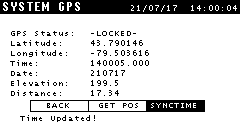
\includegraphics[width=0.49\textwidth]{figures/gps_time_synced}
  \caption{Синхронизированное время GPS}
  \label{fig:gps_time_synced}
\end{figure}

\subsection{Настройка длительности оповещения}

Длительность оповещения (в секундах)~-- это период времени, в течение которого
стрелки горизонтирования мигают красным цветом, свидетельствуя о том, что измерение
выполнено. Для редактирования длительности оповещения, наведите курсор на пункт
\textbf{Alert Length} (изображение внизу слева) и нажмите кнопку \textbf{Enter}.
Откроется экран, показанный справа:

\begin{figure}[H]
  \centering
  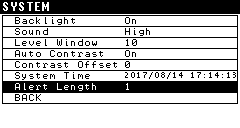
\includegraphics[width=0.49\textwidth]{figures/the_alert_length_editing_screen_1}
  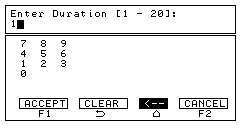
\includegraphics[width=0.49\textwidth]{figures/the_alert_length_editing_screen_2}
  \caption{Экран редактирования длительности оповещения}
  \label{fig:the_alert_length_editing_screen}
\end{figure}

Длительность оповещения может принимать любое значение в интервале от 1 секунды
до 20 секунд.

Введите желаемое значение задержки длины предупреждения с помощью экранной
клавиатуры, как описано в разделе
\nameref{subsubsec:entering_a_value_with_onscreen_keypad}.

\subsection{Назначение функций для кнопок F1 и F2}

Пользовательские функции для пунктов меню главного экрана могут быть назначены
пользователем кнопкам F1 и F2.

Чтобы назначить функцию кнопке \textbf{F1}, переместите курсор на клавишу
\textbf{F1} (изображение внизу слева) и нажмите кнопку \textbf{Enter}. Появится
экран справа:

Переместите курсор на желаемую функцию для быстрого доступа и нажмите
кнопку \textbf{Enter}.

Чтобы покинуть это экранное изображение без изменений:
\begin{itemize}
  \item наведите курсор на пункт \textbf{CANCEL}, после чего нажмите кнопку
    \textbf{Enter}, или

  \item нажмите кнопку \textbf{Back}.
\end{itemize}

\begin{figure}[H]
  \centering
  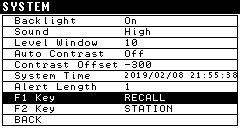
\includegraphics[width=0.49\textwidth]{figures/assigning_a_shortcut_to_the_f1_button_1}
  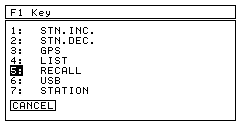
\includegraphics[width=0.49\textwidth]{figures/assigning_a_shortcut_to_the_f1_button_2}
  \caption{Назначение функции кнопке F1}
  \label{fig:assigning_a_shortcut_to_the_f1_button}
\end{figure}

Выполните ту же процедуру, чтобы назначить функцию кнопке F2.

\section{Настройки параметров съёмки}

Чтобы получить доступ к экранному изображению настройки параметров съёмки,
наведите курсор на пункт \textbf{SURVEY} (изображение внизу слева) и нажмите кнопку
\textbf{Enter}. Откроется экран, показанный справа:

\begin{figure}[H]
  \centering
  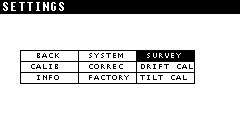
\includegraphics[width=0.49\textwidth]{figures/the_survey_setting_screen_1}
  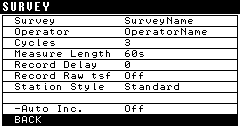
\includegraphics[width=0.49\textwidth]{figures/the_survey_setting_screen_2}
  \caption{Экран настройки параметров съёмки}
  \label{fig:the_survey_setting_screen}
\end{figure}

\subsection{Редактирование названия съёмки}

Чтобы изменить название съёмки, наведите курсор на пункт \textbf{Survey}
(изображение внизу слева) и нажмите кнопку \textbf{Enter}. Откроется экран,
показанный справа:

\newpage
\begin{figure}[H]
  \centering
  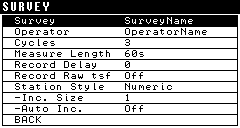
\includegraphics[width=0.49\textwidth]{figures/the_survey_name_editing_screen_1}
  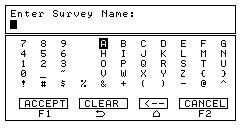
\includegraphics[width=0.49\textwidth]{figures/the_survey_name_editing_screen_2}
  \caption{Экран редактирования названия съёмки}
  \label{fig:the_survey_name_editing_screen}
\end{figure}

Название съёмки может представлять собой ту или иную комбинацию
буквенно-цифровых символов числом до 31.

Введите желаемое название съёмки с помощью экранной клавиатуры, как описано
в разделе \nameref{subsubsec:entering_a_value_with_onscreen_keypad}.

\subsection{Редактирование имени оператора}

Чтобы изменить имя оператора, наведите курсор на пункт \textbf{Operator}
(изображение внизу слева) и нажмите кнопку \textbf{Enter}. Откроется экран,
показанный справа:

\begin{figure}[H]
  \centering
  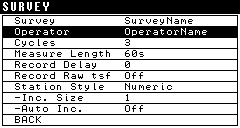
\includegraphics[width=0.49\textwidth]{figures/the_operator_name_editing_screen_1}
  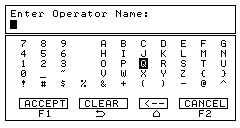
\includegraphics[width=0.49\textwidth]{figures/the_operator_name_editing_screen_2}
  \caption{Экран редактирования имени оператора}
  \label{fig:the_operator_name_editing_screen}
\end{figure}

Имя оператора может представлять собой комбинацию буквенно-цифровых
символов числом до 31 знака.

Введите желаемое имя оператора с экранной клавиатуры, как описано в разделе
\nameref{subsubsec:entering_a_value_with_onscreen_keypad}.

\subsection{Настройка числа циклов}
\label{subsec:adjusting_the_number_of_cycles}

Для настройки числа циклов измерения на вашем пункте наблюдения наведите курсор
на строку \textbf{Cycles} (изображение внизу слева) и нажмите кнопку
\textbf{Enter}.  Откроется экран, показанный справа:

\begin{figure}[H]
  \centering
  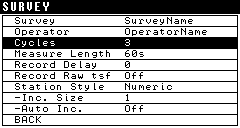
\includegraphics[width=0.49\textwidth]{figures/the_cycles_screen_1}
  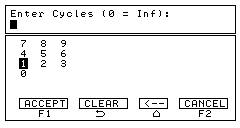
\includegraphics[width=0.49\textwidth]{figures/the_cycles_screen_2}
  \caption{Экран циклов}
  \label{fig:the_cycles_screen}
\end{figure}

\infobox{
  Число циклов определяется как количество успешных повторений отсчётов прибора
  на данном пункте наблюдения. Этот параметр может принимать любое значение в
  интервале от 1 до бесконечности, по вашему выбору. Число циклов, равное 0,
  соответствует бесконечности. Это значит, что гравиметр переведён в режим
  циклической работы, и будет выполнять измерения до тех пор, пока процесс
  снятия показаний не будет остановлен оператором.
}

Введите желаемое количество циклов с помощью экранной клавиатуры, как
описано в разделе \nameref{subsubsec:entering_a_value_with_onscreen_keypad}.

\subsection{Выбор длительности цикла измерения}
\label{subsec:adjusting_the_measurement_cycle_length}

Чтобы задать длительность одного измерения, наведите курсор на пункт
\textbf{Measure Length} (изображение внизу слева) и нажмите кнопку
\textbf{Enter}. Откроется экран, показанный справа:

\newpage
\begin{figure}[H]
  \centering
  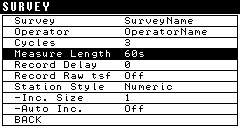
\includegraphics[width=0.49\textwidth]{figures/the_measure_length_screen_1}
  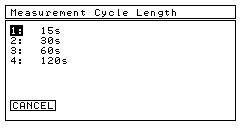
\includegraphics[width=0.49\textwidth]{figures/the_measure_length_screen_2}
  \caption{Экран выбора длительности измерения}
  \label{fig:the_measure_length_screen}
\end{figure}

Длительность измерения можно задать равной 15 секундам, 30 секундам, 60 секундам
или 120 секундам. Наведите курсор на нужное значение и нажмите кнопку
\textbf{Enter}.

Чтобы покинуть это экранное изображение без изменений:
\begin{itemize}
  \item наведите курсор на пункт \textbf{CANCEL}, после чего нажмите кнопку
    \textbf{Enter}, или

  \item нажмите кнопку \textbf{Back}.
\end{itemize}

\subsection{Корректировка задержки записи}

Вы можете ввести величину задержки записи в секундах~-- начало регистрации
данных будет отложено на это время. Это удобно при работе в поле, или во время
проверки калибровки дрейфа, когда вы хотите отложить начало снятия измерений.

Для редактирования величины задержки записи, наведите курсор на пункт
\textbf{Record Delay} (изображение внизу слева) и нажмите кнопку \textbf{Enter}.
Откроется экран, показанный справа:

\begin{figure}[H]
  \centering
  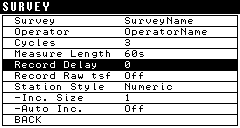
\includegraphics[width=0.49\textwidth]{figures/the_record_delay_editing_screen_1}
  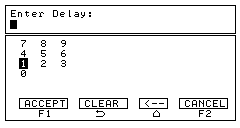
\includegraphics[width=0.49\textwidth]{figures/the_record_delay_editing_screen_2}
  \caption{Экран редактирования задержки записи}
  \label{fig:the_record_delay_editing_screen}
\end{figure}

Задержка записи может принимать любое значение от 0 до бесконечности, по
вашему выбору.

Введите значение задержки записи с экранной клавиатуры, как описано в разделе
\nameref{subsubsec:entering_a_value_with_onscreen_keypad}.

\subsection{Включение/выключение функции записи файла исходных данных TSF}

У вас есть возможность активизировать или отключить функцию записи файла
исходных данных .tsf (в дополнение к файлу фильтрованных данных .dat, который
записывается всегда).

Наведите курсор на пункт \textbf{Record Raw tsf} и нажмите кнопку
\textbf{Enter}. На дисплее появится следующее экранное изображение:

Чтобы активизировать (on) или отключить (off) функцию записи файла исходных
данных .tsf, наведите курсор на пункт \textbf{Record Raw tsf} (изображение внизу
слева) и нажмите кнопку \textbf{Enter}. Откроется экран, показанный справа:

\begin{figure}[H]
  \centering
  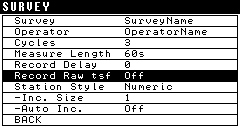
\includegraphics[width=0.49\textwidth]{figures/the_tsf_recording_screen_1}
  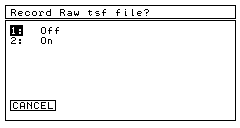
\includegraphics[width=0.49\textwidth]{figures/the_tsf_recording_screen_2}
  \caption{Экран записи файла tsf}
  \label{fig:the_tsf_recording_screen}
\end{figure}

Наведите курсор на символ 1 или 2 и нажмите кнопку \textbf{Enter}.

Чтобы покинуть это экранное изображение без изменений:
\begin{itemize}
  \item наведите курсор на пункт \textbf{CANCEL}, после чего нажмите кнопку
    \textbf{Enter}, или

  \item нажмите кнопку \textbf{Back}.
\end{itemize}

\subsection{Изменение стиля представления пункта наблюдения}

Для того, чтобы изменить стиль представления пункта наблюдения, наведите курсор
на пункт \textbf{Station Style} (изображение внизу слева) и нажмите кнопку
\textbf{Enter}.

Откроется экран, показанный справа:

\begin{figure}[H]
  \centering
  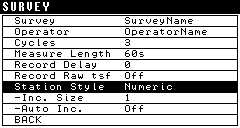
\includegraphics[width=0.49\textwidth]{figures/the_station_style_editing_screen_1}
  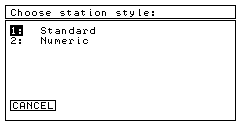
\includegraphics[width=0.49\textwidth]{figures/the_station_style_editing_screen_2}
  \caption{Экран редактирования стиля пункта наблюдения}
  \label{fig:the_station_style_editing_screen}
\end{figure}

Стиль представления пункта наблюдения может быть стандартным
(\textbf{Standard}), т.~е., представлять собой любое буквенно-цифровое
наименование, или цифровым (\textbf{Numeric}). Наведите курсор на символ 1 или 2
и нажмите кнопку \textbf{Enter}.

В зависимости от выбранного вами стиля представления пункта наблюдения, меню
съёмки будет немного отличаться, как показано на рисунке внизу.

\begin{figure}[H]
  \centering
  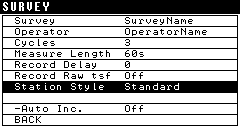
\includegraphics[width=0.49\textwidth]{figures/station_style_standard_vs_numeric_1}
  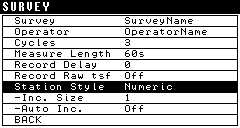
\includegraphics[width=0.49\textwidth]{figures/station_style_standard_vs_numeric_2}
  \caption{Стили представления пункта наблюдения: Standard и Numeric}
  \label{fig:station_style_standard_vs_numeric}
\end{figure}

Как можно заметить, параметр <<Inc. Size>> появляется только, когда выбран
цифровой стиль представления пункта наблюдения.

\subsection{Выбор шага приращения (только для цифрового стиля)}

Чтобы изменить величину шага приращения, наведите курсор на пункт \textbf{-Inc.
  Size} (изображение внизу слева) и нажмите кнопку \textbf{Enter}. Откроется
экран, показанный справа:

\begin{figure}[H]
  \centering
  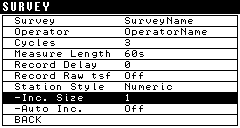
\includegraphics[width=0.49\textwidth]{figures/the_increment_size_screen_1}
  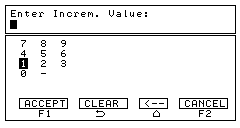
\includegraphics[width=0.49\textwidth]{figures/the_increment_size_screen_2}
  \caption{Экран выбора шага приращения}
  \label{fig:the_increment_size_screen}
\end{figure}

Введите размер приращения с экранной клавиатуры, как описано в разделе
\nameref{subsubsec:entering_a_value_with_onscreen_keypad}.

Чтобы покинуть это экранное изображение без изменений:
\begin{itemize}
  \item наведите курсор на пункт \textbf{CANCEL}, после чего нажмите кнопку
    \textbf{Enter}, или

  \item нажмите кнопку \textbf{Back}.
\end{itemize}

\subsection{Включение/выключение автоматического перехода к следующему пункту}

Функция \textbf{Auto station increment} автоматически переводит ваш прибор CG-6
к следующему пункту наблюдения после выполнения всех циклов измерения на текущем
пункте наблюдения.

В числовом стиле станции новое имя станции будет представлять собой значение
текущей станции плюс размер приращения.

В стандартном стиле станции имя новой станции будет следующей станцией в
предварительно установленном списке станций. Широта, долгота, высота и номер
линии станции также будут обновлены соответственно.

Чтобы включить или отключить автоматическое приращение станции, переместите
курсор на \textbf{-Auto Inc} (изображение внизу слева) и нажмите кнопку
\textbf{Enter}. Появится экран справа:

\begin{figure}[H]
  \centering
  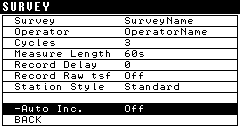
\includegraphics[width=0.49\textwidth]{figures/the_automatic_increment_screen_1}
  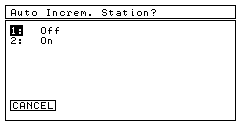
\includegraphics[width=0.49\textwidth]{figures/the_automatic_increment_screen_2}
  \caption{Экран функции автоматического перехода}
  \label{fig:the_automatic_increment_screen}
\end{figure}

Наведите курсор на символ 1 или 2 и нажмите кнопку \textbf{Enter}.

Чтобы покинуть это экранное изображение без изменений:
\begin{itemize}
  \item наведите курсор на пункт \textbf{CANCEL}, после чего нажмите кнопку
    \textbf{Enter}, или

  \item нажмите кнопку \textbf{Back}.
\end{itemize}

\section{Просмотр и изменение параметров калибровки}

На экранном изображении Settings наведите курсор на пункт \textbf{CALIB}
(изображение внизу слева) и нажмите кнопку \textbf{Enter}. Откроется экран,
показанный справа:

\begin{figure}[H]
  \centering
  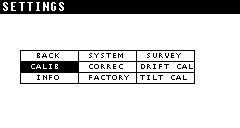
\includegraphics[width=0.49\textwidth]{figures/the_instrument_parameter_screen_1}
  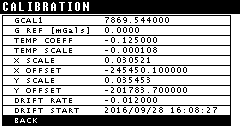
\includegraphics[width=0.49\textwidth]{figures/the_instrument_parameter_screen_2}
  \caption{Экран параметров прибора}
  \label{fig:the_instrument_parameter_screen}
\end{figure}

\newpage
\warningbox{
  Параметры прибора задаются на заводе-изготовителе Scintrex, и они
  индивидуальны для каждого гравиметра \cg{}:

  \begin{itemize}
    \item В обычных условиях оператор не должен изменять параметры
      \textbf{TEMP COEFF} и \textbf{TEMP SCALE}

    \item Параметр \textbf{GCAL1} может быть изменён только в случае повторной
      калибровки прибора \cg{}

    \item Параметр \textbf{DRIFT RATE} изменяется после проверки калибровки
      дрейфа

    \item Параметр \textbf{DRIFT START} может быть изменён в любое время, но
      обычно после проверки калибровки дрейфа

    \item Параметры \textbf{X SCALE}, \textbf{X OFFSET}, \textbf{Y SCALE},
      \textbf{Y OFFSET} изменяются после проверки калибровки дрейфа

    \item Параметр \textbf{G REF} может быть изменён в любое время в случае
      необходимости
  \end{itemize}
}

\subsection[Изменение постоянной гравиметра]{Изменение постоянной гравиметра GCAL1}

Чтобы изменить постоянную гравиметра \textbf{GCAL1}, наведите курсор на пункт
GCAL1 (изображение внизу слева) и нажмите кнопку \textbf{Enter}. Откроется
экран, показанный справа:

\begin{figure}[H]
  \centering
  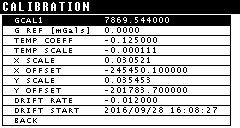
\includegraphics[width=0.49\textwidth]{figures/the_gcal1_editing_screen_1}
  \includegraphics[width=0.49\textwidth]{figures/the_gcal1_editing_screen_2}
  \caption{Экран редактирования GCAL1}
  \label{fig:the_gcal1_editing_screen}
\end{figure}

Величина GCAL1 задаётся на заводе-изготовителе, и в обычных условиях изменять её
не следует.

Однако, если вы решите перекалибровать свой \cg{}, новое значение GCAL1 можно
будет ввести с экранной клавиатуры, как описано в разделе
\nameref{subsubsec:entering_a_value_with_onscreen_keypad}.

Чтобы покинуть это экранное изображение без изменений:
\begin{itemize}
  \item наведите курсор на пункт \textbf{CANCEL}, после чего нажмите кнопку
    \textbf{Enter}, или

  \item нажмите кнопку \textbf{Back}.
\end{itemize}

\subsection{Изменение опорной величины силы тяжести}

Чтобы отредактировать опорную величину силы тяжести, наведите курсор на пункт
\textbf{G REF} (изображение внизу слева) и нажмите кнопку \textbf{Enter}.
Откроется экран, показанный справа:

\begin{figure}[H]
  \centering
  \includegraphics[width=0.49\textwidth]{figures/the_gravity_reference_value_editing_screen_1}
  \includegraphics[width=0.49\textwidth]{figures/the_gravity_reference_value_editing_screen_2}
  \caption{Экран редактирования опорной величины силы тяжести}
  \label{fig:the_gravity_reference_value_editing_screen}
\end{figure}

Опорная величина силы тяжести может принимать любое значение в диапазоне от 0 до
8000 мГал. Эта величина вычитается из текущего показания силы тяжести.

Введите новое значение величины опорной силы тяжести с помощью экранной
клавиатуры, как описано в разделе
\nameref{subsubsec:entering_a_value_with_onscreen_keypad}.

Чтобы покинуть это экранное изображение без изменений:
\begin{itemize}
  \item наведите курсор на пункт \textbf{CANCEL}, после чего нажмите кнопку
    \textbf{Enter}, или

  \item нажмите кнопку \textbf{Back}.
\end{itemize}

\subsection{Изменение температурного коэффициента}

\warningbox{
  В обычных условиях оператор не должен изменять величину параметра \textbf{TEMP
    COEFF}.
}

Чтобы изменить величину температурного коэффициента, наведите курсор на пункт
\textbf{TEMP COEFF} (изображение внизу слева) и нажмите кнопку \textbf{Enter}.
Откроется экран, показанный справа:

\begin{figure}[H]
  \centering
  \includegraphics[width=0.49\textwidth]{figures/the_temperature_coefficient_editing_screen_1}
  \includegraphics[width=0.49\textwidth]{figures/the_temperature_coefficient_editing_screen_2}
  \caption{Экран редактирования температурного коэффициента}
  \label{fig:the_temperature_coefficient_editing_screen}
\end{figure}

Температурный коэффициент является отрицательной величиной в диапазоне от
\textminus{}0,1 до \textminus{}0,2.

Введите новый температурный коэффициент с помощью экранной клавиатуры, как
описано в разделе \nameref{subsubsec:entering_a_value_with_onscreen_keypad}.

Чтобы покинуть это экранное изображение без изменений:
\begin{itemize}
  \item наведите курсор на пункт \textbf{CANCEL}, после чего нажмите кнопку
    \textbf{Enter}, или

  \item нажмите кнопку \textbf{Back}.
\end{itemize}

\subsection[Изменение коэффициента усиления по температуре]{Изменение коэффициента усиления по температуре (TEMP SCALE)}

\warningbox{
  В обычных условиях оператор не должен изменять величину параметра \textbf{TEMP
    SCALE}.
}

Чтобы изменить величину коэффициента усиления по температуре, наведите курсор на
пункт \textbf{TEMP SCALE} (изображение внизу слева) и нажмите кнопку
\textbf{Enter}.  Откроется экран, показанный справа:

\begin{figure}[H]
  \centering
  \includegraphics[width=0.49\textwidth]{figures/the_temperature_gain_editing_screen_1}
  \includegraphics[width=0.49\textwidth]{figures/the_temperature_gain_editing_screen_2}
  \caption{Экран редактирования коэффициента усиления по температуре}
  \label{fig:the_temperature_gain_editing_screen}
\end{figure}

Введите новое значение прироста температуры с помощью экранной клавиатуры,
как описано в разделе \nameref{subsubsec:entering_a_value_with_onscreen_keypad}.

Чтобы покинуть это экранное изображение без изменений:
\begin{itemize}
  \item наведите курсор на пункт \textbf{CANCEL}, после чего нажмите кнопку
    \textbf{Enter}, или

  \item нажмите кнопку \textbf{Back}.
\end{itemize}

\subsection{Изменение постоянных датчика наклона}

\infobox{Обычно новые постоянные датчика наклона вводятся автоматически при
  проведении проверки калибровки уровня, как описывается далее в этой главе.
  Показанные ниже действия позволяют вам вручную изменить постоянные датчика
  наклона в случае необходимости.}

Постоянные датчика наклона включают в себя: X Scale, X Offset, Y Scale и Y Offset.

Чтобы редактировать эти постоянные, наведите курсор на соответствующее поле
(изображение внизу слева) и нажмите кнопку \textbf{Enter}. Откроется экран,
показанный справа:

\newpage
\begin{figure}[H]
  \centering
  \includegraphics[width=0.49\textwidth]{figures/the_x_level_scale_editing_screen_1}
  \includegraphics[width=0.49\textwidth]{figures/the_x_level_scale_editing_screen_2}
  \caption{Экран редактирования шкалы уровня по оси X}
  \label{fig:the_x_level_scale_editing_screen}
\end{figure}

\begin{figure}[H]
  \centering
  \includegraphics[width=0.49\textwidth]{figures/the_x_level_offset_editing_screen_1}
  \includegraphics[width=0.49\textwidth]{figures/the_x_level_offset_editing_screen_2}
  \caption{Экран редактирования смещения уровня по оси X}
  \label{fig:the_x_level_offset_editing_screen}
\end{figure}

\begin{figure}[H]
  \centering
  \includegraphics[width=0.49\textwidth]{figures/the_y_level_scale_editing_screen_1}
  \includegraphics[width=0.49\textwidth]{figures/the_y_level_scale_editing_screen_2}
  \caption{Экран редактирования шкалы уровня по оси Y}
  \label{fig:the_y_level_scale_editing_screen}
\end{figure}

\begin{figure}[H]
  \centering
  \includegraphics[width=0.49\textwidth]{figures/the_y_level_offset_editing_screen_1}
  \includegraphics[width=0.49\textwidth]{figures/the_y_level_offset_editing_screen_2}
  \caption{Экран редактирования смещения уровня по оси Y}
  \label{fig:the_y_level_offset_editing_screen}
\end{figure}

С помощью экранной клавиатуры введите новое значение, как описано в разделе
\nameref{subsubsec:entering_a_value_with_onscreen_keypad}.

Чтобы покинуть это экранное изображение без изменений:
\begin{itemize}
  \item наведите курсор на пункт \textbf{CANCEL}, после чего нажмите кнопку
    \textbf{Enter}, или

  \item нажмите кнопку \textbf{Back}.
\end{itemize}

\subsection{Изменение величины дрейфа}

\warningbox{
  Изменение скорости дрейфа или времени начала дрейфа приведёт к изменению ваших
  данных.
}

\infobox{
  Обычно новое значение величины дрейфа вводится автоматически при проведении
  проверки калибровки дрейфа, как описывается далее в этой главе.  Показанные
  ниже действия позволяют вам вручную изменить скорость дрейфа в случае
  необходимости.
}

Для редактирования величины скорости дрейфа, наведите курсор на пункт
\textbf{DRIFT RATE} (изображение внизу слева) и нажмите кнопку Enter. Откроется
экран, показанный справа:

\newpage
\begin{figure}[H]
  \centering
  \includegraphics[width=0.49\textwidth]{figures/the_drift_rate_editing_screen_1}
  \includegraphics[width=0.49\textwidth]{figures/the_drift_rate_editing_screen_2}
  \caption{Экран редактирования величины дрейфа}
  \label{fig:the_drift_rate_editing_screen}
\end{figure}

Введите новую скорость дрейфа с экранной клавиатуры, как описано в
\nameref{subsubsec:entering_a_value_with_onscreen_keypad}.

Чтобы покинуть это экранное изображение без изменений:
\begin{itemize}
  \item наведите курсор на пункт \textbf{CANCEL}, после чего нажмите кнопку
    \textbf{Enter}, или

  \item нажмите кнопку \textbf{Back}.
\end{itemize}

\subsection{Изменение времени начала компенсации дрейфа}

Время начала компенсации дрейфа~-- это момент времени, начиная с которого
производится компенсация дрейфа вашего прибора \cg{}. Это может быть любая дата в
интервале от прошлого до настоящего.

Для редактирования времени начала компенсации дрейфа, наведите курсор на пункт
\textbf{DRIFT START} (изображение внизу слева) и нажмите кнопку \textbf{Enter}.
Откроется экран, показанный справа:

\infobox{
  Вы можете вручную синхронизировать время начала компенсации дрейфа по
  юлианскому времени, используя для этого планшетный компьютер. Эта процедура
  более подробно описана в руководстве по программному обеспечению LynxLG (p/n
  115370003).
}

Для редактирования времени начала компенсации дрейфа, наведите курсор на пункт
\textbf{DRIFT START} (изображение внизу слева) и нажмите кнопку \textbf{Enter}.
Откроется экран, показанный справа:

\begin{figure}[H]
  \centering
  \includegraphics[width=0.49\textwidth]{figures/the_drift_start_time_editing_screen_1}
  \includegraphics[width=0.49\textwidth]{figures/the_drift_start_time_editing_screen_2}
  \caption{Экран редактирования времени начала дрейфа}
  \label{fig:the_drift_start_time_editing_screen}
\end{figure}

Чтобы ввести год, наведите курсор на пункт \textbf{Year} (изображение внизу слева) и
нажмите кнопку \textbf{Enter}. Откроется экран, показанный справа:

\begin{figure}[H]
  \centering
  \includegraphics[width=0.49\textwidth]{figures/the_year_editing_screen_1}
  \includegraphics[width=0.49\textwidth]{figures/the_year_editing_screen_2}
  \caption{Экран редактирования года}
  \label{fig:the_year_editing_screen_1}
\end{figure}

Введите год с экранной клавиатуры, как описано в разделе
\nameref{subsubsec:entering_a_value_with_onscreen_keypad}.

Чтобы покинуть это экранное изображение без изменений:
\begin{itemize}
  \item наведите курсор на пункт \textbf{CANCEL}, после чего нажмите кнопку
    \textbf{Enter}, или

  \item нажмите кнопку \textbf{Back}.
\end{itemize}

Аналогичную процедуру нужно выполнить, чтобы отредактировать месяц, день, час,
минуты и секунды.

\section{Поправки к показаниям прибора}

В вашем приборе \cg{} вы можете активизировать или отключить функцию введения
поправок на температуру, дрейф, земные приливы или на наклон.

На экранном изображении Settings наведите курсор на пункт \textbf{CORREC}
(изображение внизу слева) и нажмите кнопку \textbf{Enter}. Откроется экран,
показанный справа:

\begin{figure}[H]
  \centering
  \includegraphics[width=0.49\textwidth]{figures/the_instrument_corrections_screen_1}
  \includegraphics[width=0.49\textwidth]{figures/the_instrument_corrections_screen_2}
  \caption{Экран поправок к показаниям прибора}
  \label{fig:the_instrument_corrections_screen}
\end{figure}

\subsection{Включение/выключение поправки за температуру}

Чтобы активизировать или отключить поправку за температуру, наведите курсор на
пункт \textbf{Temperature} (изображение внизу слева) и нажмите кнопку
\textbf{Enter}. Откроется экран, показанный справа:

\begin{figure}[H]
  \centering
  \includegraphics[width=0.49\textwidth]{figures/the_temperature_correction_screen_1}
  \includegraphics[width=0.49\textwidth]{figures/the_temperature_correction_screen_2}
  \caption{Экран поправки на температуру}
  \label{fig:the_temperature_correction_screen}
\end{figure}

Чтобы активизировать (\textbf{On}) или отключить (\textbf{Off}) поправку за
температуру, наведите курсор на символ 1 или 2 и нажмите кнопку \textbf{Enter}.

Чтобы покинуть это экранное изображение без изменений:
\begin{itemize}
  \item наведите курсор на пункт \textbf{CANCEL}, после чего нажмите кнопку
    \textbf{Enter}, или

  \item нажмите кнопку \textbf{Back}.
\end{itemize}

\subsection{Включение/выключение поправки за земные приливы}

Чтобы активизировать или отключить поправку за земные приливы, наведите курсор
на пункт \textbf{Tide} (изображение внизу слева) и нажмите кнопку
\textbf{Enter}. Откроется экран, показанный справа:

\begin{figure}[H]
  \centering
  \includegraphics[width=0.49\textwidth]{figures/the_tide_correction_screen_1}
  \includegraphics[width=0.49\textwidth]{figures/the_tide_correction_screen_2}
  \caption{Экран поправки на земные приливы}
  \label{fig:the_tide_correction_screen}
\end{figure}

Чтобы активизировать (\textbf{On}) или отключить (\textbf{Off}) поправку за
земные приливы, наведите курсор на символ 1 или 2 и нажмите кнопку
\textbf{Enter}.

Чтобы покинуть это экранное изображение без изменений:
\begin{itemize}
  \item наведите курсор на пункт \textbf{CANCEL}, после чего нажмите кнопку
    \textbf{Enter}, или

  \item нажмите кнопку \textbf{Back}.
\end{itemize}

\subsection{Включение/выключение поправки на наклон}

Чтобы активизировать или отключить поправку на наклон, наведите курсор на пункт
\textbf{Level} (изображение внизу слева) и нажмите кнопку \textbf{Enter}.
Откроется экран, показанный справа:

\begin{figure}[H]
  \centering
  \includegraphics[width=0.49\textwidth]{figures/the_tilt_correction_screen_1}
  \includegraphics[width=0.49\textwidth]{figures/the_tilt_correction_screen_2}
  \caption{Экран поправки на наклон}
  \label{fig:the_tilt_correction_screen}
\end{figure}

Чтобы активизировать (\textbf{On}) или отключить (\textbf{Off}) поправку на
наклон, наведите курсор на символ 1 или 2 и нажмите кнопку \textbf{Enter}.

Чтобы покинуть это экранное изображение без изменений:
\begin{itemize}
  \item наведите курсор на пункт \textbf{CANCEL}, после чего нажмите кнопку
    \textbf{Enter}, или

  \item нажмите кнопку \textbf{Back}.
\end{itemize}

Чтобы вернуться к экрану настроек:
\begin{itemize}
  \item переместите курсор на назад \textbf{BACK} и нажмите кнопку
    \textbf{Enter}, или

  \item нажмите кнопку \textbf{Back}.
\end{itemize}

\section{Проверка калибровки дрейфа}

Время от времени вы можете захотеть уточнить коэффициент компенсации дрейфа
вашего \cg{}.

\warningbox{
  Прибор \cg{} должен находиться в нерабочем режиме, т.~е., прежде чем
  выполнять проверку калибровки дрейфа, необходимо остановить регистрацию
  данных. Более того, длительность измерения должна быть задана равной 60
  секундам, а число циклов должно быть задано равным как минимум 240 циклам
  (т.~е., проверка калибровки дрейфа продолжается 4 часа). Проверку
  предпочтительно проводить в ночное время.
}

Чтобы получить доступ к экрану проверки калибровки дрейфа, наведите курсор на
пункт \textbf{DRIFT CAL} (изображение внизу слева) и нажмите кнопку
\textbf{Enter}. Откроется экран, показанный справа:

\begin{figure}[H]
  \centering
  \includegraphics[width=0.49\textwidth]{figures/the_drift_calibration_test_screen_befor_started_1}
  \includegraphics[width=0.49\textwidth]{figures/the_drift_calibration_test_screen_befor_started_2}
  \caption{Экран проверки калибровки дрейфа: перед началом}
  \label{fig:the_drift_calibration_test_screen_befor_started}
\end{figure}

Установите прибор \cg{} по уровню, согласно указаниям раздела
\nameref{subsec:leveling_the_cg6_autograv} на
странице~\pageref{subsec:leveling_the_cg6_autograv}. После того, как обе стрелки
горизонтирования станут зелёными, вы можете приступать к проведению проверки
калибровки дрейфа.

Чтобы начать проверку калибровки дрейфа, наведите курсор на пункт \textbf{START}
и нажмите кнопку \textbf{Enter} (левый экран). Теперь прибор \cg{} находится в
режиме проверки калибровки дрейфа. Откроется экран, показанный справа:

\begin{figure}[H]
  \centering
  \includegraphics[width=0.49\textwidth]{figures/the_drift_calibration_test_screen_test_in_progress_1}
  \includegraphics[width=0.49\textwidth]{figures/the_drift_calibration_test_screen_test_in_progress_2}
  \caption{Экран проверки калибровки дрейфа: в процессе проверки}
  \label{fig:the_drift_calibration_test_screen_test_in_progress}
\end{figure}

По завершении первого цикла появится следующее экранное изображение:

\begin{figure}[H]
  \centering
  \includegraphics[width=0.49\textwidth]{figures/the_drift_calibration_test_active_screen_first_cycle_completed}
  \caption{Экран проверки калибровки дрейфа: первый цикл завершён}
  \label{fig:the_drift_calibration_test_active_screen_first_cycle_completed}
\end{figure}

Чтобы прекратить проверку калибровки дрейфа, вы можете дать прибору \cg{} самому
закончить проверку калибровки дрейфа, выполнив определённое число циклов, или
можете навести курсор на пункт END TEST и нажать кнопку \textbf{Enter}.

На дисплее появится следующее экранное изображение:

\begin{figure}[H]
  \centering
  \includegraphics[width=0.49\textwidth]{figures/the_drift_calibration_test_screen_test_completed}
  \caption{Экран проверки калибровки дрейфа: проверка завершена}
  \label{fig:the_drift_calibration_test_screen_test_completed}
\end{figure}

Новое значение скорости дрейфа показано ниже текущей скорости дрейфа. Чтобы
принять новое значение скорости дрейфа, наведите курсор на ячейку
\textbf{ACCEPT} и нажмите кнопку \textbf{Enter}. В экранном изображении на
рисунке~\ref{fig:the_drift_calibration_test_screen_accepting_new_result}
показано обновлённое значение скорости дрейфа.

\begin{figure}[H]
  \centering
  \includegraphics[width=0.49\textwidth]{figures/the_drift_calibration_test_screen_accepting_new_result}
  \caption{Экран проверки калибровки дрейфа: новый результат принят}
  \label{fig:the_drift_calibration_test_screen_accepting_new_result}
\end{figure}

Если вы решите не принимать новое значение скорости дрейфа, наведите курсор на
пункт \textbf{QUIT} и нажмите кнопку \textbf{Enter}.

Вы вернётесь к экранному изображению Settings.

После завершения проверки калибровки дрейфа будет автоматически создан файл
дрейфа (с расширением .drift). Чтобы обратиться к этому файлу, выполняйте
указания раздела \nameref{subsec:taking_a_measurement} на
странице~\pageref{subsec:taking_a_measurement}. На
рисунке~\ref{fig:the_drift_file_under_root_folder} показано расположение файла
дрейфа в памяти прибора \cg{}:

\begin{figure}[H]
  \centering
  \includegraphics[width=0.7\textwidth]{figures/the_drift_file_under_root_folder}
  \caption{}Корневая папка с файлом дрейфа
  \label{fig:the_drift_file_under_root_folder}
\end{figure}

На следующем изображении показан типичный файл дрейфа.

\begin{figure}[H]
  \centering
  \includegraphics[width=\textwidth]{figures/the_drift_file}
  \caption{Файл дрейфа}
  \label{fig:the_drift_file}
\end{figure}

\section{Проверка калибровки уровня}

Время от времени у вас может возникнуть необходимость в корректировке масштаба и
величины смещения датчиков наклона в вашем приборе \cg{}.

\warningbox{
  Поставьте гравиметр \cg{} на устойчивую поверхность и убедитесь, что
  прибор находится в нерабочем режиме, т.~е., регистрация данных должна быть
  остановлена.  Задайте длительность измерения равной 30 секундам (рекомендуемое
  значение, но в случае необходимости можно использовать и другие значения этого
  параметра).
}

Чтобы получить доступ к экрану проверки наклона, наведите курсор на пункт
\textbf{TILT CAL} (изображение внизу слева) и нажмите кнопку \textbf{Enter}.
Откроется экран, показанный справа:

\begin{figure}[H]
  \centering
  \includegraphics[width=0.49\textwidth]{figures/the_level_calibration_test_screen_1}
  \includegraphics[width=0.49\textwidth]{figures/the_level_calibration_test_screen_2}
  \caption{Экран проверки калибровки уровня}
  \label{fig:the_level_calibration_test_screen}
\end{figure}

Установите прибор \cg{} по уровню, согласно указаниям раздела
\nameref{subsec:leveling_the_cg6_autograv} на странице
\pageref{subsec:leveling_the_cg6_autograv}. После того, как обе стрелки
горизонтирования станут зелёными, вы можете приступать к проведению проверки
уровня.

Наведите курсор на пункт \textbf{START} (изображение внизу слева) и нажмите кнопку
\textbf{Enter}. Откроется экран, показанный справа:

\begin{figure}[H]
  \centering
  \includegraphics[width=0.49\textwidth]{figures/the_level_calibration_test_screen_in_setup_mode_1}
  \includegraphics[width=0.49\textwidth]{figures/the_level_calibration_test_screen_in_setup_mode_2}
  \caption{Экран проверки калибровки уровня в режиме настройки}
  \label{fig:the_level_calibration_test_screen_in_setup_mode}
\end{figure}

Отгоризонтируйте прибор \cg{} до 0 угловых секунд по осям X и Y и нажмите
кнопку \textbf{Enter}. На дисплее появится следующее экранное изображение:

\newpage
\begin{figure}[H]
  \centering
  \includegraphics[width=0.49\textwidth]{figures/the_level_calibration_test_screen_in_collecting_mode_point_1}
  \caption{Экран калибровки уровня в режиме сбора данных, точка 1}
  \label{fig:the_level_calibration_test_screen_in_collecting_mode_point_1}
\end{figure}

Сейчас ваш прибор \cg{} находится в режиме сбора данных. В конце цикла (30 секунд)
появится следующее экранное изображение:

\begin{figure}[H]
  \centering
  \includegraphics[width=0.49\textwidth]{figures/the_level_calibration_test_screen_at_the_end_of_the_point_1}
  \caption{Экран проверки калибровки уровня в конце точки 1}
  \label{fig:the_level_calibration_test_screen_at_the_end_of_the_point_1}
\end{figure}

Следуйте указаниям для следующих настроек уровня: (200, 0), (\textminus{}200,
0), (0, 200), (\textminus{}200, 0) and (0, 0).

В конце замера (0, 0) появится следующее экранное изображение:

\begin{figure}[H]
  \centering
  \includegraphics[width=0.49\textwidth]{figures/the_level_clibration_test_screen_at_the_end_of_point_6}
  \caption{Экран проверки калибровки уровня в конце точки 6}
  \label{fig:the_level_clibration_test_screen_at_the_end_of_point_6}
\end{figure}

Чтобы принять новые значения масштаба и смещения наклона, наведите курсор на
ячейку \textbf{ACCEPT} и нажмите кнопку \textbf{Enter}.

Чтобы выйти, не принимая новые значения масштаба и смещения наклона,
наведите курсор на ячейку \textbf{QUIT} и нажмите кнопку \textbf{Enter}.

Чтобы заново провести калибровочную проверку уровня, наведите курсор на пункт
\textbf{RESTART}, после чего нажмите кнопку \textbf{Enter}.

После завершения проверки калибровки уровня автоматически создаётся файл
калибровки уровня (с расширением .level). Чтобы обратиться к этому файлу,
выполняйте указания раздела \nameref{subsec:taking_a_measurement} на
странице~\pageref{subsec:taking_a_measurement}. На показанных далее изображениях
видно расположение файла калибровки уровня в памяти прибора \cg{}:

\begin{figure}[H]
  \centering
  \includegraphics[width=0.7\textwidth]{figures/the_level_calibration_file_under_root_folder}
  \caption{Корневая папка с файлом калибровки уровня}
  \label{fig:the_level_calibration_file_under_root_folder}
\end{figure}

Следующий рисунок иллюстрирует типичный файл дрейфа:

\begin{figure}[H]
  \centering
  \includegraphics[width=\textwidth]{figures/the_level_calibration_file}
  \caption{Файл калибровки уровня}
  \label{fig:the_level_calibration_file}
\end{figure}

\section{Информация о системе}

Для доступа к экранному изображению системной информации, наведите курсор на
пункт \textbf{INFO} и нажмите кнопку \textbf{Enter}. На дисплее появится
следующее экранное изображение:

\begin{figure}[H]
  \centering
  \includegraphics[width=0.49\textwidth]{figures/the_system_information_screen}
  \caption{Экран системной информации}
  \label{fig:the_system_information_screen}
\end{figure}

На экранном изображении системной информации можно увидеть следующее: серийный
номер вашего прибора \cg{}, версию аппаратно-программного обеспечения, процент
используемой памяти и температура датчика (в \textcelsius{}) и её отклонение от
заданного значения (в мК). Диапазон отклонения от заданного значения составляет
\textpm{}1000 мК.

\warningbox{
  Заводское меню доступно только инженерам компании Scintrex.
}

\section[Настройка списка пунктов]{Настройка предварительно составленного списка пунктов наблюдения}
\label{sec:setting_up_the_pre-set_list_of_stations}

Для просмотра предварительно составленного списка пунктов наблюдения зайдите в
главное экранное изображение и наведите курсор на пункт \textbf{LIST}
(изображение внизу слева), после чего нажмите кнопку \textbf{Enter}. Откроется
показанное справа экранное изображение, содержащее предварительно составленный
список пунктов наблюдения:

\newpage
\begin{figure}[H]
  \centering
  \includegraphics[width=0.49\textwidth]{figures/pre-set_list_of_stations_1}
  \includegraphics[width=0.49\textwidth]{figures/pre-set_list_of_stations_2}
  \caption{Предварительно составленный список пунктов наблюдения}
  \label{fig:pre-set_list_of_stations}
\end{figure}

Предварительно составленный список пунктов наблюдения хранится в файле
<<\textbf{stations.txt}>>, в корневой папке гравиметра \cg{}. Вы можете
просмотреть и отредактировать этот файл, активизировав режим USB в вашем
гравиметре \cg{}, и подключив кабель USB-А к разъёму USB-B (\textnumero{} 200239)
на гравиметре \cg{} и разъём USB-A к разъёмам на вашем портативном компьютере или
на планшете.

Для доступа к режиму USB зайдите в главное экранное изображение и наведите
курсор на пункт \textbf{USB} (изображение внизу слева), после чего нажмите
кнопку \textbf{Enter}.  Откроется экран, показанный справа:

\begin{figure}[H]
  \centering
  \includegraphics[width=0.49\textwidth]{figures/entering_usb_mode_1}
  \includegraphics[width=0.49\textwidth]{figures/entering_usb_mode_2}
  \caption{Вход в режим USB}
  \label{fig:entering_usb_mode}
\end{figure}

\warningbox{
  Прибор \cg{} должен находиться в нерабочем режиме, т.~е., прежде чем режим
  устройства USB, необходимо остановить регистрацию данных.
}

Тогда ваш прибор \cg{} воспринимается компьютером как запоминающее устройство
большой ёмкости. Теперь вы можете без труда выполнять различные операции с
файлом, например, скопировать его на флэш-накопитель USB. В корневом каталоге
находится файл stations.txt, как показано на рисунке внизу.

\begin{figure}[H]
  \centering
  \includegraphics[width=0.7\textwidth]{figures/stations.txt_file_in_usb_mode}
  \caption{Файл stations.txt в режиме USB}
  \label{fig:stations.txt_file_in_usb_mode}
\end{figure}

\begin{figure}[H]
  \centering
  \includegraphics[width=0.49\textwidth]{figures/default_stations.txt_file}
  \caption{Стандартный файл stations.txt}
  \label{fig:default_stations.txt_file}
\end{figure}

Файл stations.txt может вмещать до 1000 пунктов наблюдения. Он поддерживает 3
формата:
\begin{itemize}
  \item StationName,Latitude,Longitude,Elevation,Line
  \item StationName,Latitude,Longitude,Elevation
  \item StationName
\end{itemize}

После отключения гравиметра CG-6 от USB, внесённые в файл stations.txt изменения
будут отражаться в меню <<LIST>>.

\infobox{
  Предварительно составленный список пунктов наблюдения доступен только в режиме
  стандартного стиля представления пунктов наблюдения. Режим цифрового
  представления пунктов наблюдения позволяет просмотреть список, но выделение
  сделать невозможно.
}

Теперь настройка вашего прибора \cg{} завершена.
